%%%%%%%%%%%%%%%%%%%%%%%%%%%%%%%%%%%%%%%%%
% University/School Laboratory Report
% LaTeX Template
% Version 4.0 (March 21, 2022)
%
% This template originates from:
% https://www.LaTeXTemplates.com
%
%%%%%%%%%%%%%%%%%%%%%%%%%%%%%%%%%%%%%%%%%

%----------------------------------------------------------------------------------------
%	PACKAGES AND DOCUMENT CONFIGURATIONS
%----------------------------------------------------------------------------------------

\documentclass[
	a4paper, % Paper size, specify a4paper (A4) or letterpaper (US letter)
	10pt, % Default font size, specify 10pt, 11pt or 12pt
]{CSUniSchoolLabReport}

\addbibresource{sample.bib} % Bibliography file (located in the same folder as the template)

%----------------------------------------------------------------------------------------
%	REPORT INFORMATION
%----------------------------------------------------------------------------------------

\title{Report 4: Partial Differential Equations (PDEs)} % Report title
\subtitle{Git: https://github.com/simonblaue/MCP-Ex4.git}

\author{Simon \textsc{Blaue}} % Author name(s), add additional authors like: '\& James \textsc{Smith}'


\date{\today} % Date of the report

%----------------------------------------------------------------------------------------

\begin{document}

\maketitle % Insert the title, author and date using the information specified above

\vspace*{40px}

\begin{tabular}{l r}
	Universität Göttingen \\ % Date the experiment was performed
	Faculty of Physics \\
	Instructor: Prof. Dr. S. Schumann \\
	Tutors: Dr. E. Bothmann, M. Knobbe \\ % Partner names
\end{tabular}


% If you need to include an abstract, uncomment the lines below
%\begin{abstract}
%	Abstract text
%\end{abstract}

\newpage
%----------------------------------------------------------------------------------------
%	CONTENT
%----------------------------------------------------------------------------------------
% \headtopline
% \headsepline

\ohead{\pagemark}
\automark{subsection}

\section{Laplace Equation}

\subsection{Iterator methods}

First lets check which method converges the fastest:

\begin{figure}[H]
	\centering
	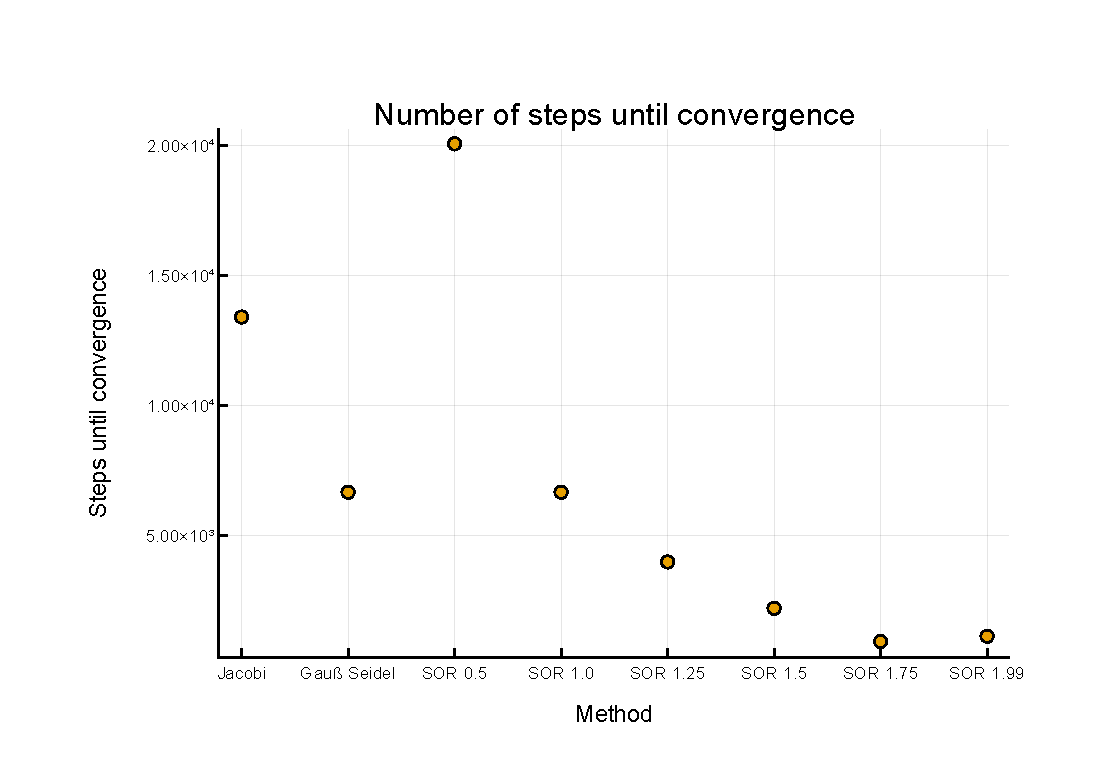
\includegraphics[width=\textwidth]{../saves_t1/number_of_convergence_steps.pdf}
	\caption{Number of steps until convergence concerning the Laplace error $\max\epsilon<1\times 10^{-3}$.}
\end{figure}

I observe that Gauß-Seidel and SOR with $\alpha=1.0$ need the same number of time steps as expected. The fastest method is SOR with  $\alpha=1.75$, because with $\alpha=1.99$ we get to close to unstable regimes. Obviously SOR with $\alpha=0.5$ takes the longest, as the updating step is damped with the factor $\alpha$. Now I will observe the evolution of the maximal error and the average error of the different methods.

\begin{figure}[H]
	\centering
	\begin{subfigure}[b]{0.49\textwidth}
			\centering
			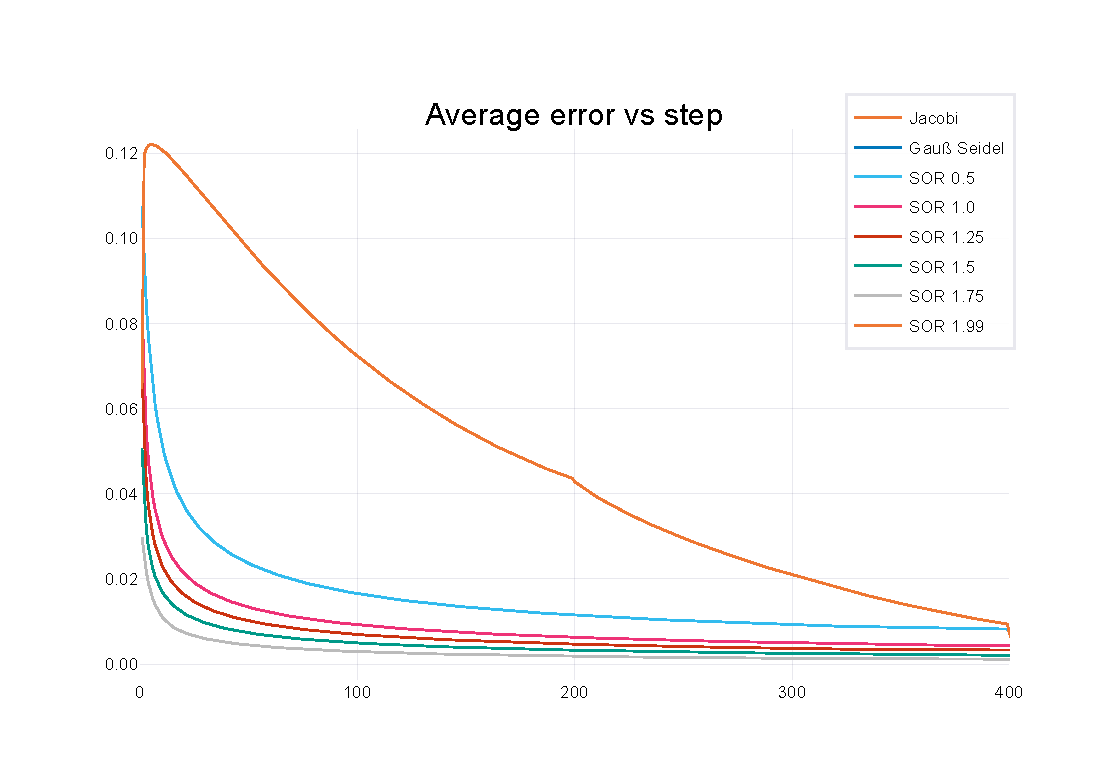
\includegraphics[width=\textwidth]{../saves_t1/av_errors_comp.pdf}
			\label{fig:av_errors}
	\end{subfigure}
	\hfill
	\begin{subfigure}[b]{0.49\textwidth}
			\centering
			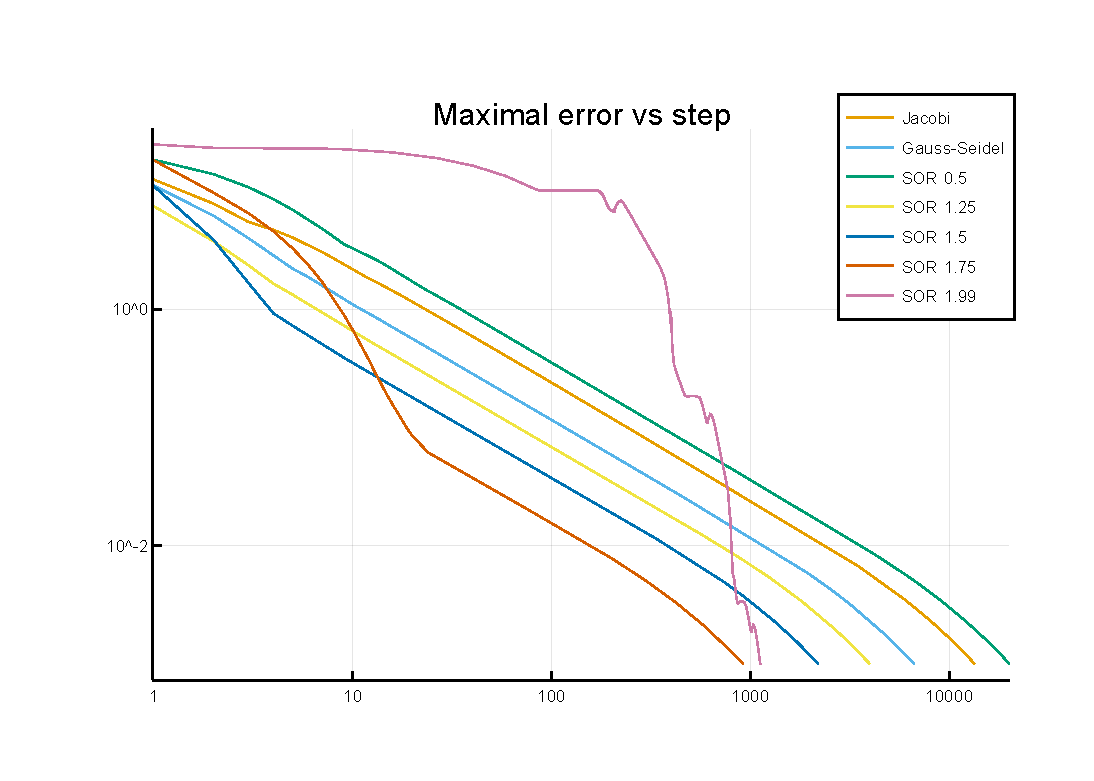
\includegraphics[width=\textwidth]{../saves_t1/max_errors_comp.pdf}
			\label{fig:max_errors}
	\end{subfigure}
	\caption{Maximal and average error for different iteration methods.}
	\label{fig:errors}
\end{figure}

As discussed before, SOR with $\alpha=1.0$ and Gauß-Seidel method are the same, hence I plotted only the latter. The error development for all methods besides SOR with$\alpha\geq 1.5$ seem qualitatively the same. However for higher $\alpha$ I observe indents in the curve, which seems to boost the algorithm. This is due to the algorithm taking bigger steps in the right direction once it found this direction. 
For $\alpha=1.99$ the curve is very rigid, and I was not sure, if it is relay converged to the right solution, hence I plotted the result below. As it turns out the method also converges to the expected result.

\begin{figure}[H]
	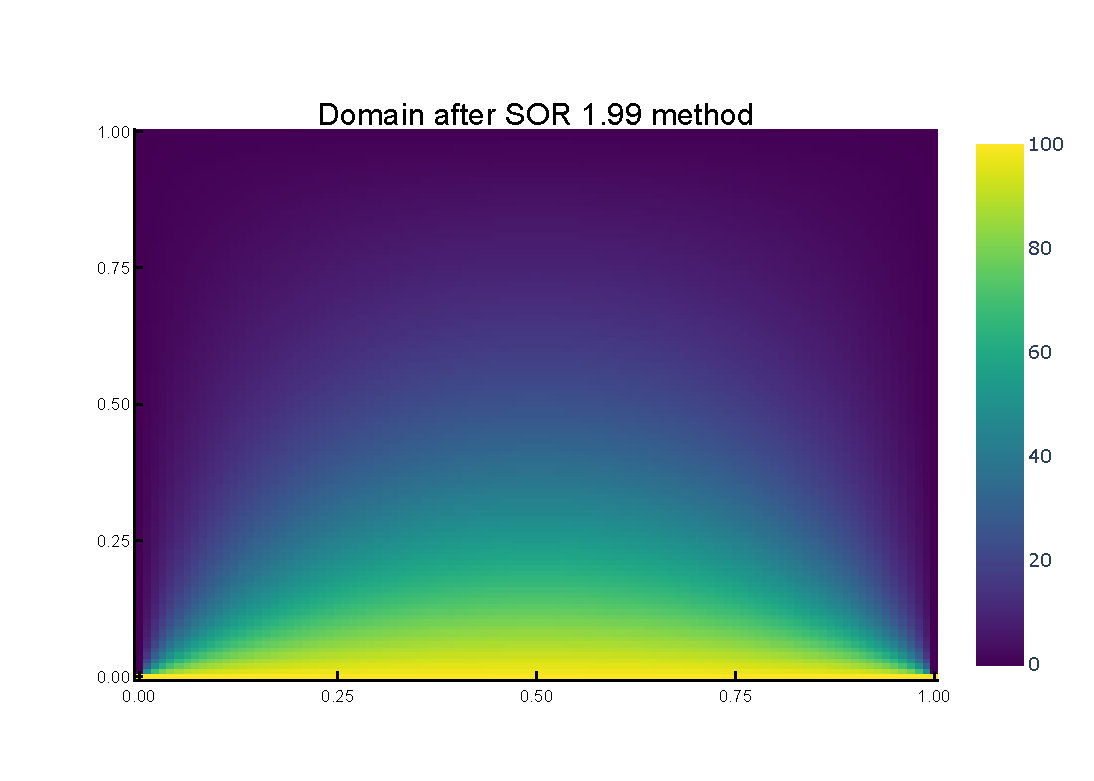
\includegraphics[width=\textwidth]{../saves_t1/sor199_heatmap.pdf}
	\caption{Domain after iterating with the SOR 1.99 method to verify right convergence.}
\end{figure}

\subsection{SOR}

The natural question to ask is what happens for an even further boosted SOR method? I found that for $\alpha = 2.0$ the algorithm does not converge in  50000 steps. It seems that it would not have converged to the right domain, as the result shows stripes and the maximal error starts to fluctuate a lot after 100 time steps. The system can not recover from that.

\begin{figure}[H]
	\centering
	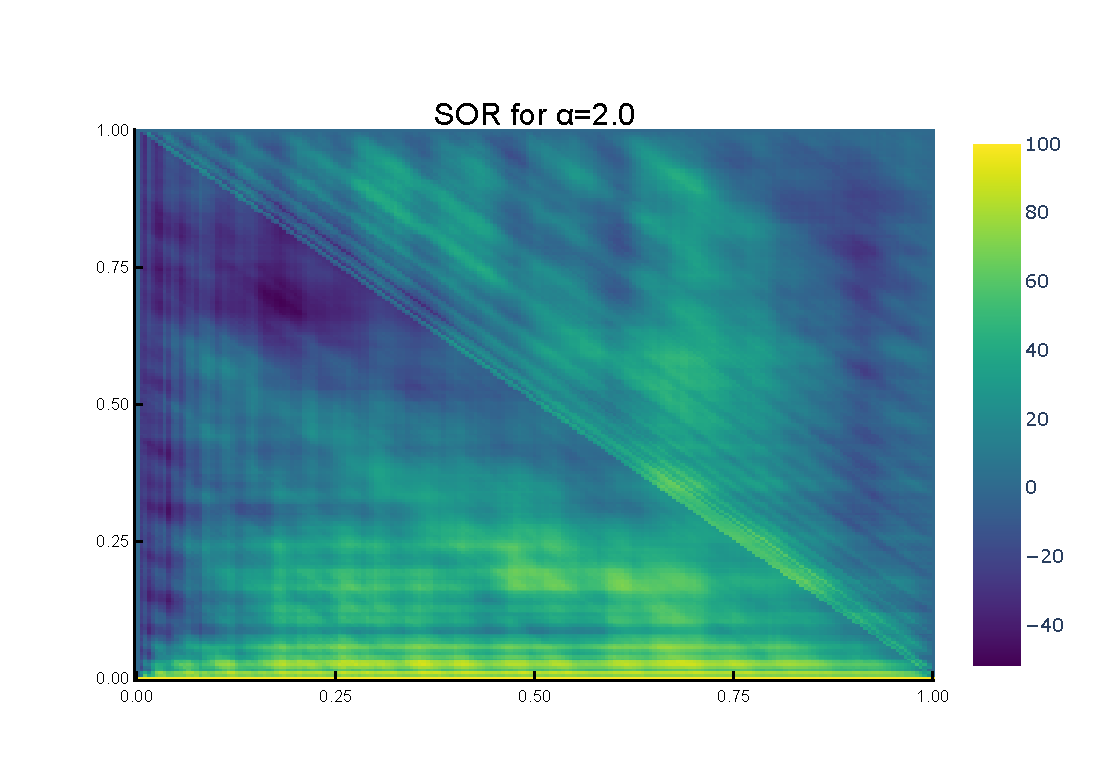
\includegraphics[width=0.9\textwidth]{../saves_t1/broken_SOR_heatmap.pdf}
\end{figure}

\begin{figure}[H]
	\centering
	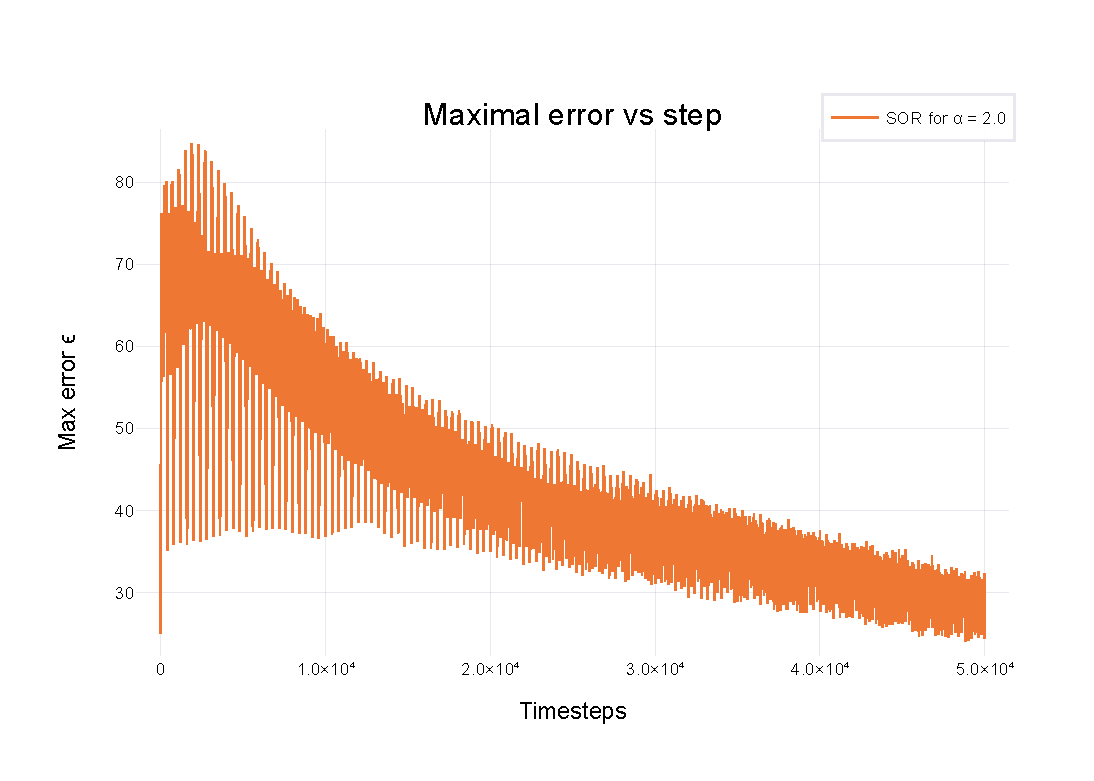
\includegraphics[width=0.9\textwidth]{../saves_t1/broken_SOR_error.pdf}
	% \caption{}
\end{figure}

\subsection{Infinite sum solution}

Now I will cross verify the iterative solution with an aproximated analytical solution. First have a look at the analytical "infinite" sum solution for different numbers of summands. 

\begin{figure}[H]
	\centering
	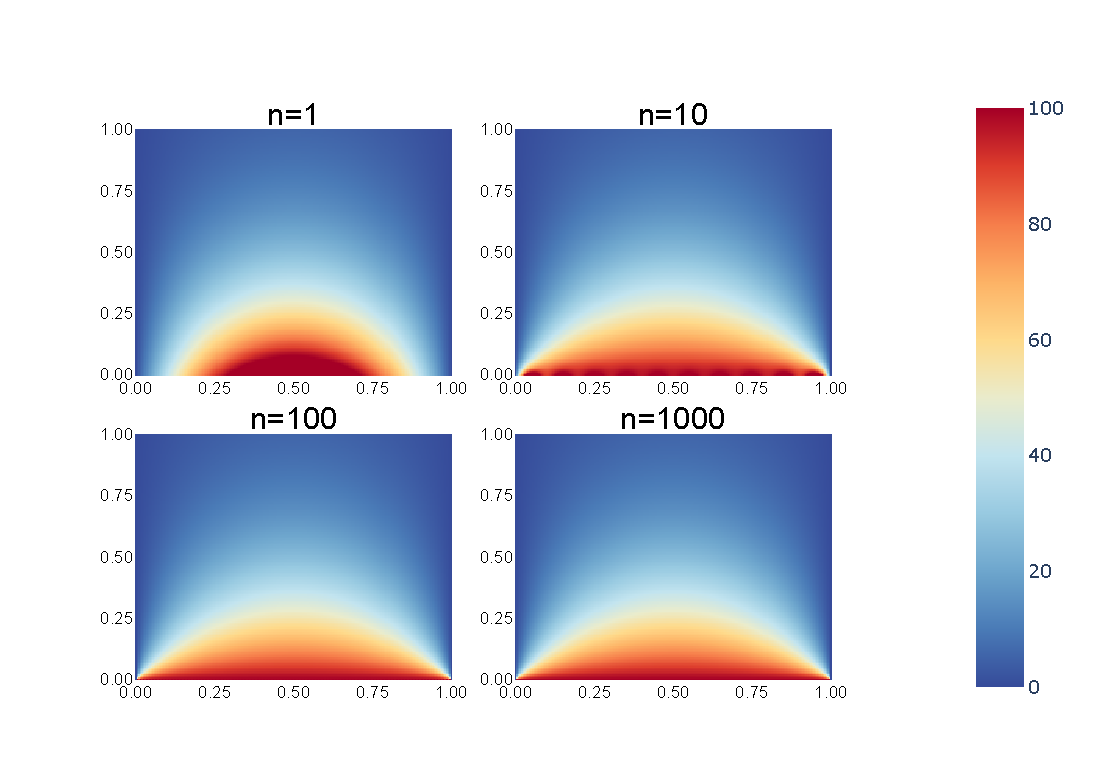
\includegraphics[width=\textwidth]{../saves_t1/comp_lapplace_series_heatmap.pdf}
	\caption{Results for the "infinite" sum solution to the Laplace equation for different numbers of terms $n$.}
\end{figure}

As I increase the number of terms more and more sine functions are added left and right to the first one, and towards the top an exponential decay fills in. Comparing the "infinite" sum solution for 1000 terms with the Gauß-Seidel method reveals that the exponential decay is to weak, or the Gauß-Seidel method did not propagate long enough. Subtracting both results displays that at the edges the solutions are identical (yellow) in the top they do not fit together as the iterative solution did not propergate that far.

\begin{figure}[H]
	\centering
	\begin{subfigure}[b]{\textwidth}
		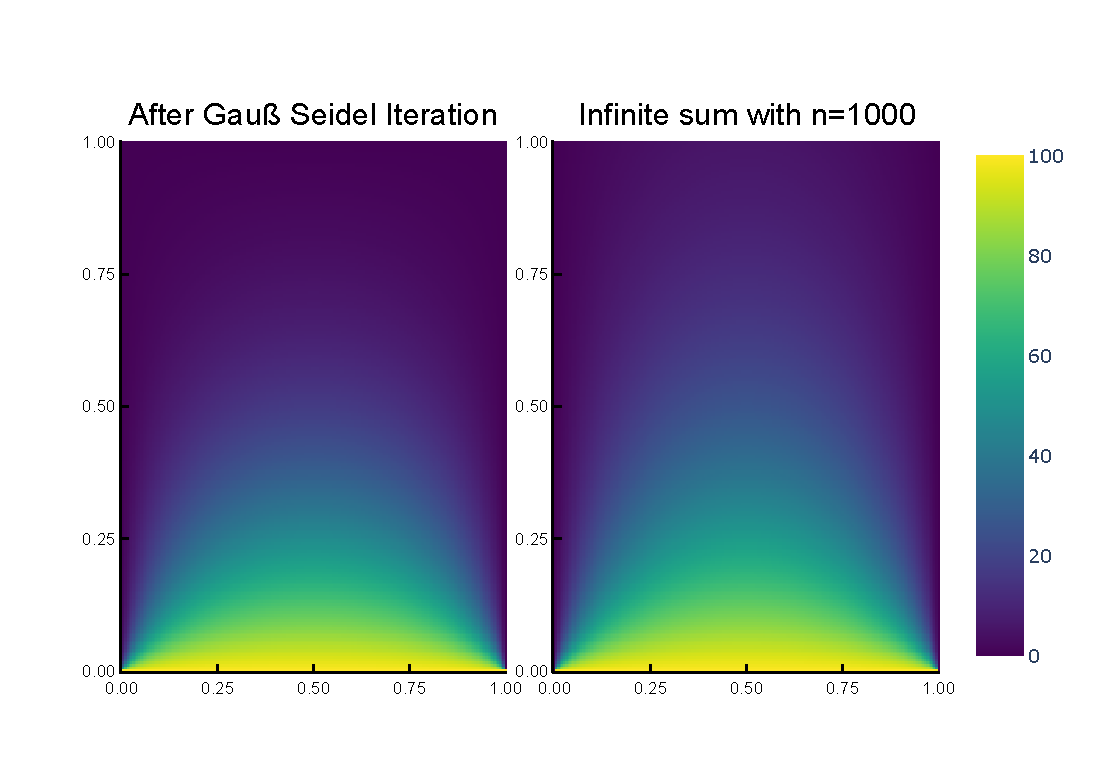
\includegraphics[width=\textwidth]{../saves_t1/comp_laplace_heatmap.pdf}
		\caption{Comparison of the infinite sum solution with 1000 terms and the Gauß Seidel iterator solution.}
	\end{subfigure}
	\hfill
	\centering
	\begin{subfigure}[b]{0.6\textwidth}
		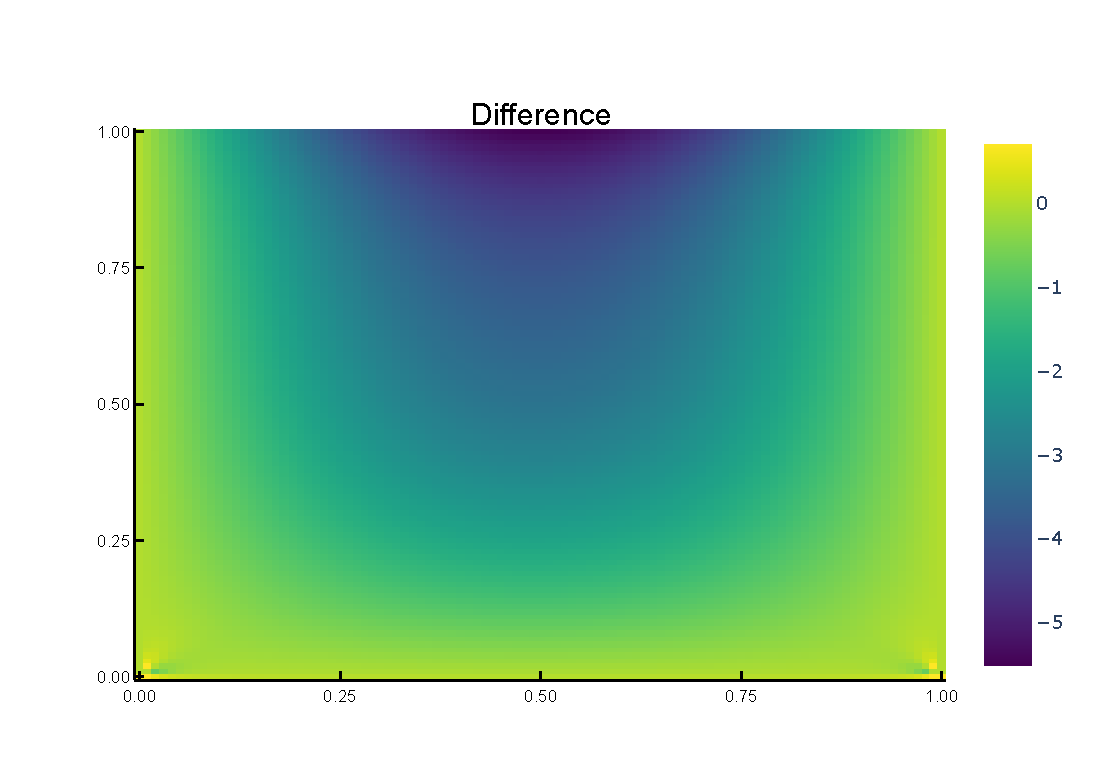
\includegraphics[width=\textwidth]{../saves_t1/difference_laplace_heatmap.pdf}
		\caption{Difference between the infinite sum solution with 1000 terms and the Gauß Seidel iterator solution.}
	\end{subfigure}
\end{figure}


\section{Diffusion}

In this task I implemented four different method for solving the diffusion equation. To varyfiy they all converged to the same solution I plotted a time evolution of all of them. The time domain is in the y-axis, the rod domain in the x-axis, displayed in \autoref{fig:comp_diff_integ}. As expected, th rod cools down, but holds the qualitative temperature profile.

\subsection{Integration methods}

\begin{figure}[H]
	\centering
	\begin{subfigure}[b]{0.49\textwidth}
		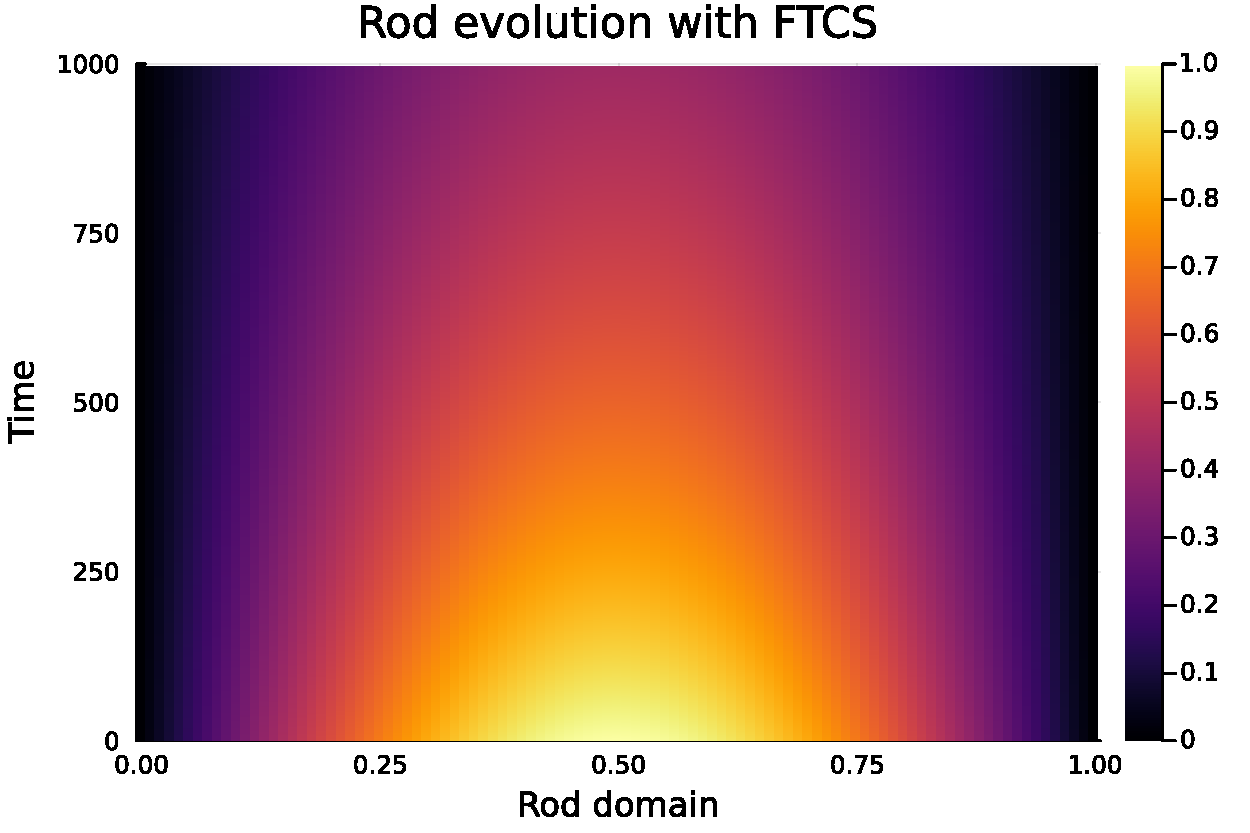
\includegraphics[width=\textwidth]{../saves_t2/rod_FTCS.pdf}
	\end{subfigure}
	\hfill
	\begin{subfigure}[b]{0.49\textwidth}
		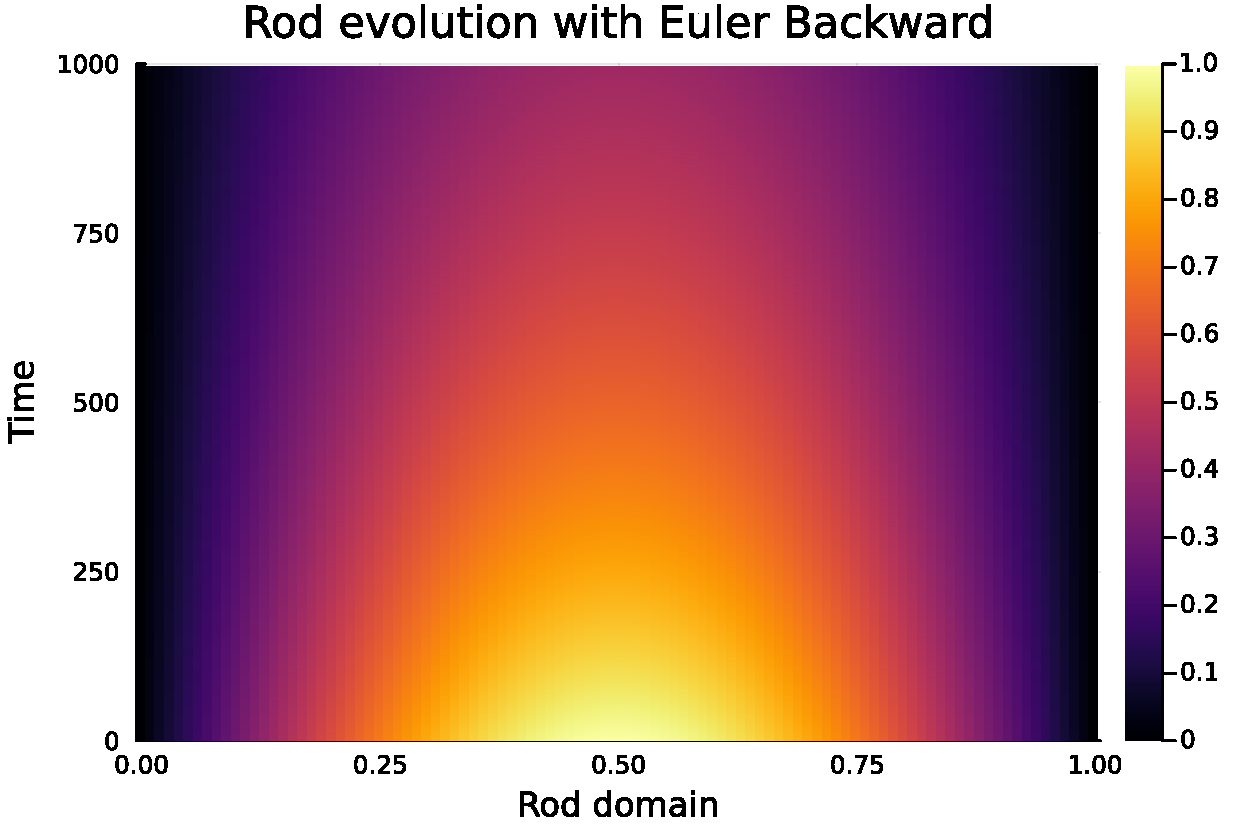
\includegraphics[width=\textwidth]{../saves_t2/rod_euler_back.pdf}
	\end{subfigure}
	\hfill
	\begin{subfigure}[b]{0.49\textwidth}
		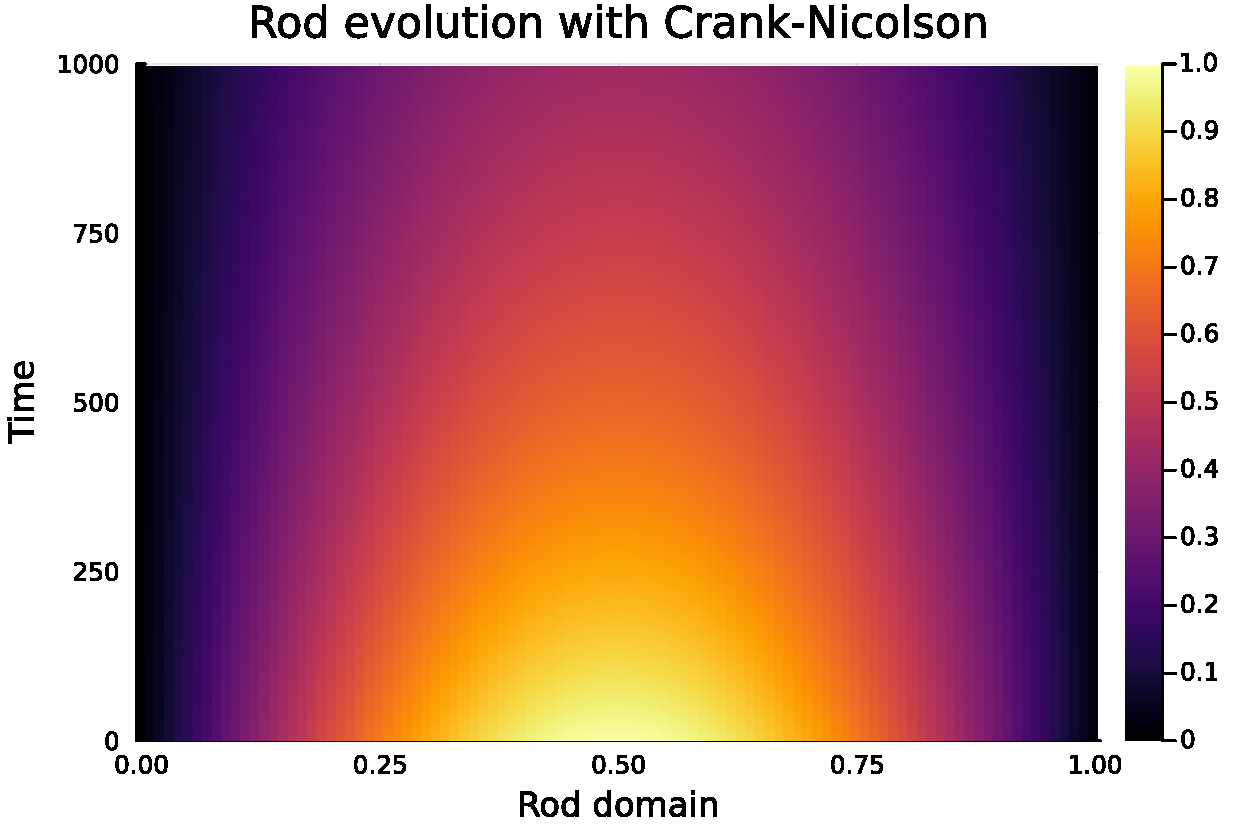
\includegraphics[width=\textwidth]{../saves_t2/rod_crank_nic.pdf}
	\end{subfigure}
	\hfill
	\begin{subfigure}[b]{0.49\textwidth}
		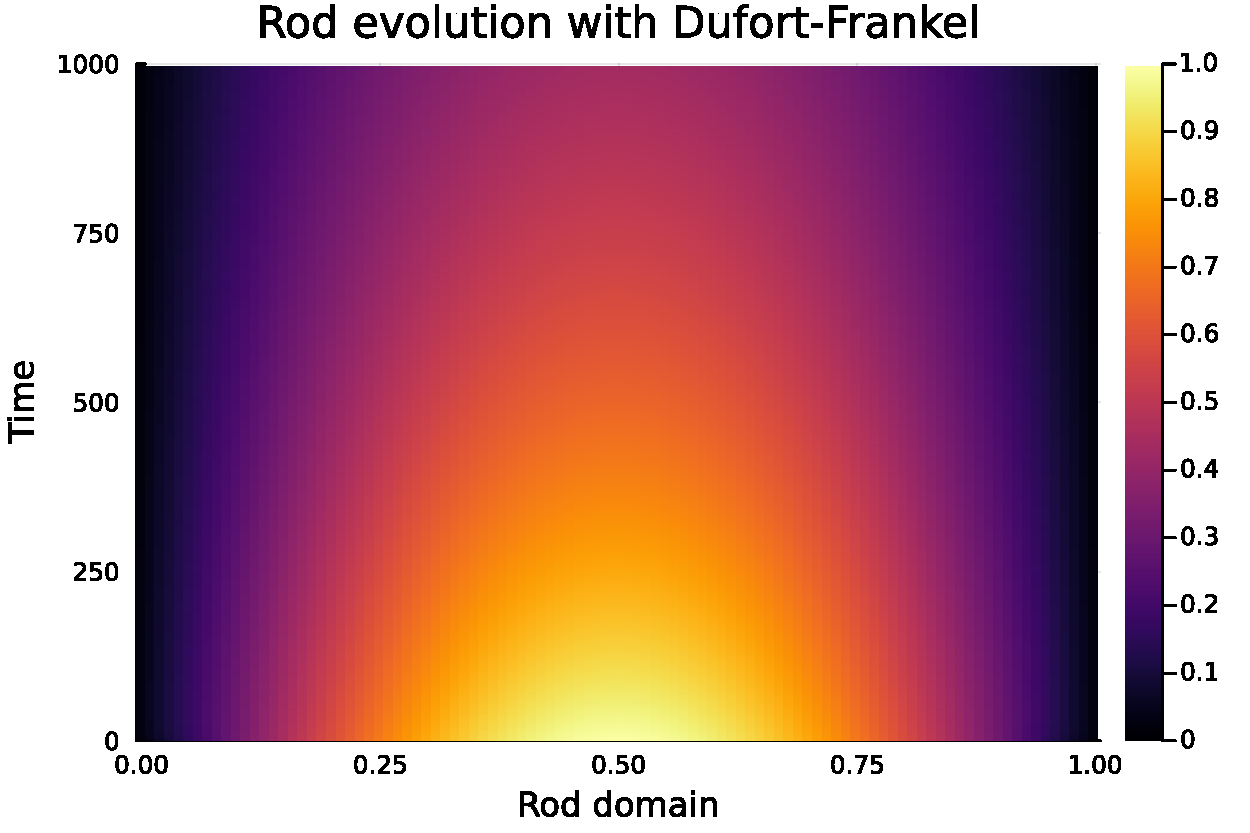
\includegraphics[width=\textwidth]{../saves_t2/rod_dufort_frankel.pdf}
	\end{subfigure}
	\hfill
	\caption{Temporal evolution of the rod's temperature along the y-axis. The evolution seems to be the same for all four integration methods.}
	\label{fig:comp_diff_integ}
\end{figure}

\subsection{Error comparison}

To investigate the stability of the different method, I plotted the error against the analytical solution for different time step widths. I expect unconditionally stability for the implicit methods Euler Backwards and Crank-Nicolson and the Dufort-Frankel method. The FCTS method is not unconditionally stable and should result in a huge error at some large enough $\Delta t$, depending on $\Delta x$ ($\Delta x = 0.01$). However also the other methods haev a time step dependent truncation error. I displayed their evolution individually in \autoref{fig:all_trunc_errors}.
For comparing the other erros I will cut off the instability of the FCTS scheme at an error of $\epsilon = 0.007$. I observe that the other schemes seem stable in the tested regime.


\begin{figure}[H]
	\centering
	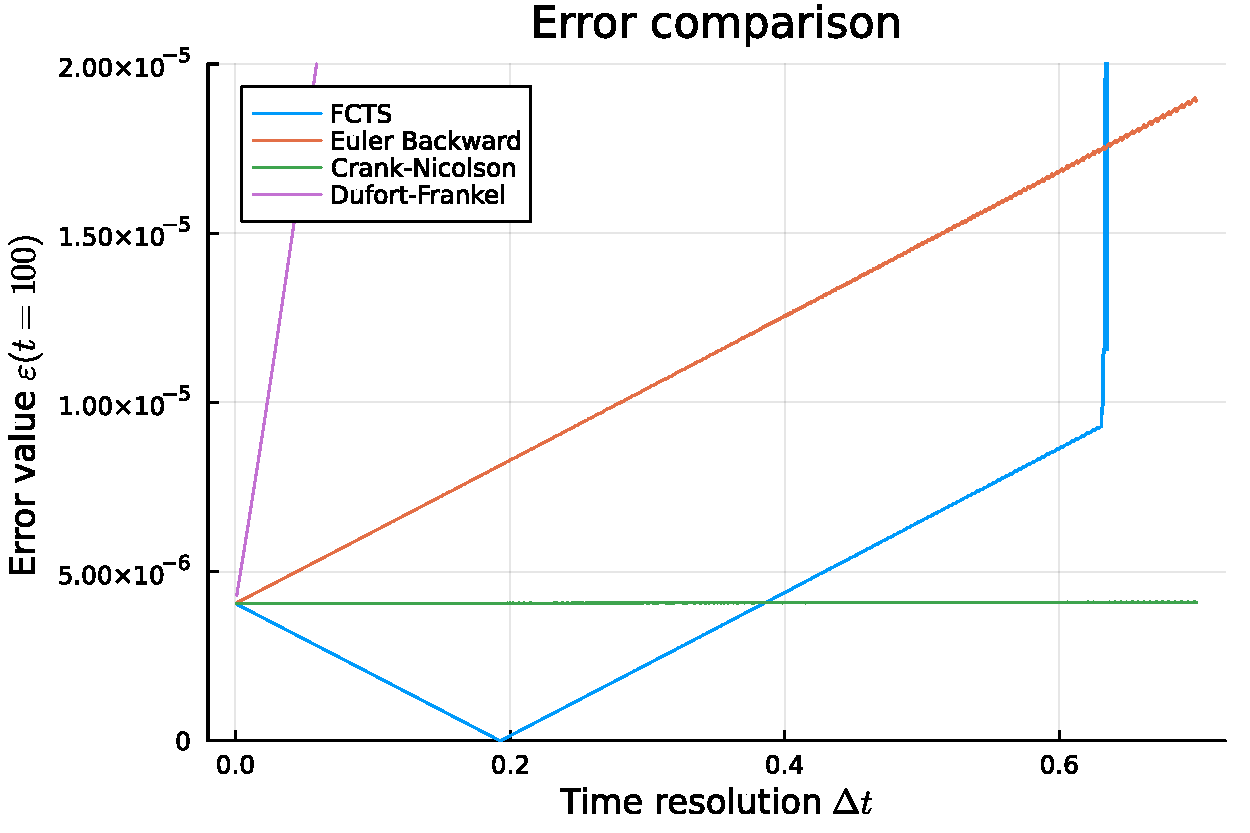
\includegraphics[width=\textwidth]{../saves_t2/error_comp_diffusion.pdf}
	\caption{Error comparison for the different methods}
\end{figure}

\begin{figure}[H]
	\centering
	\begin{subfigure}[b]{0.49\textwidth}
		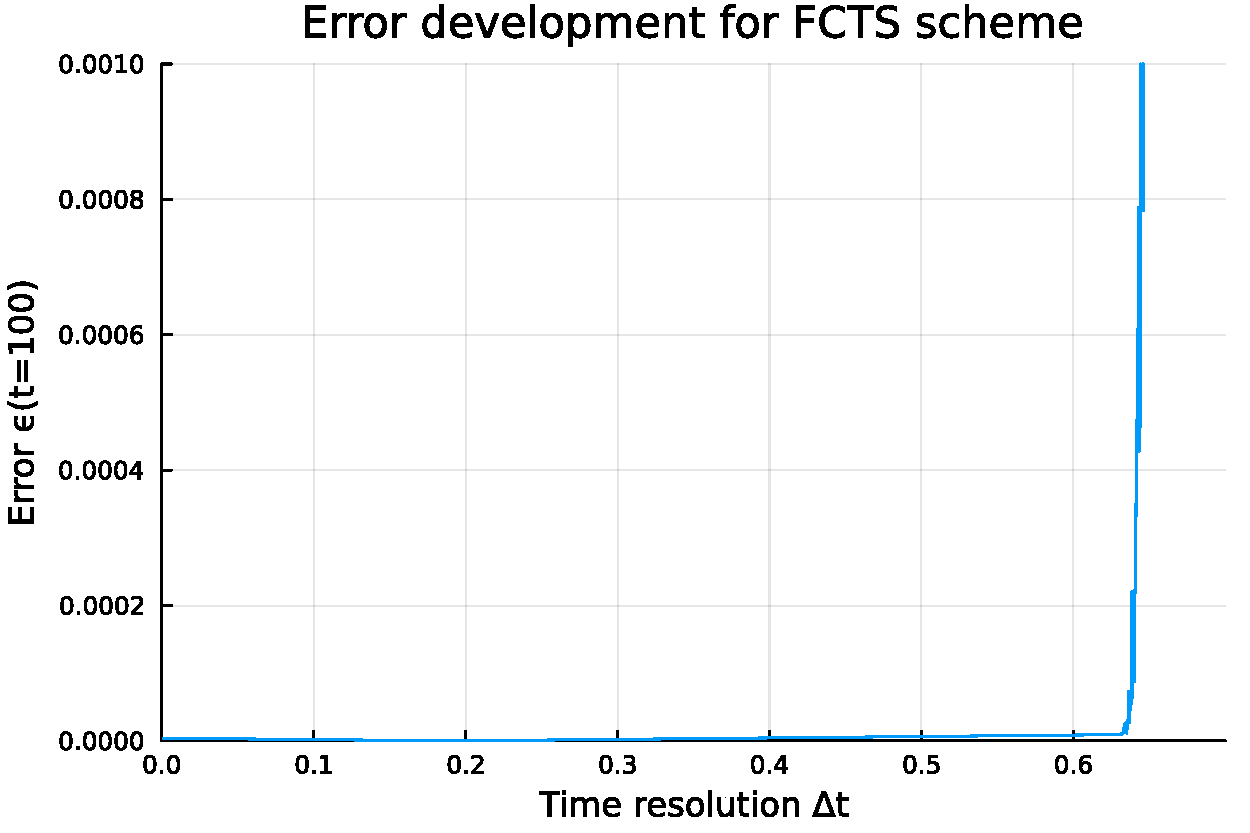
\includegraphics[width=\textwidth]{../saves_t2/error_development_fcts.pdf}
	\end{subfigure}
	\hfill
	\begin{subfigure}[b]{0.49\textwidth}
		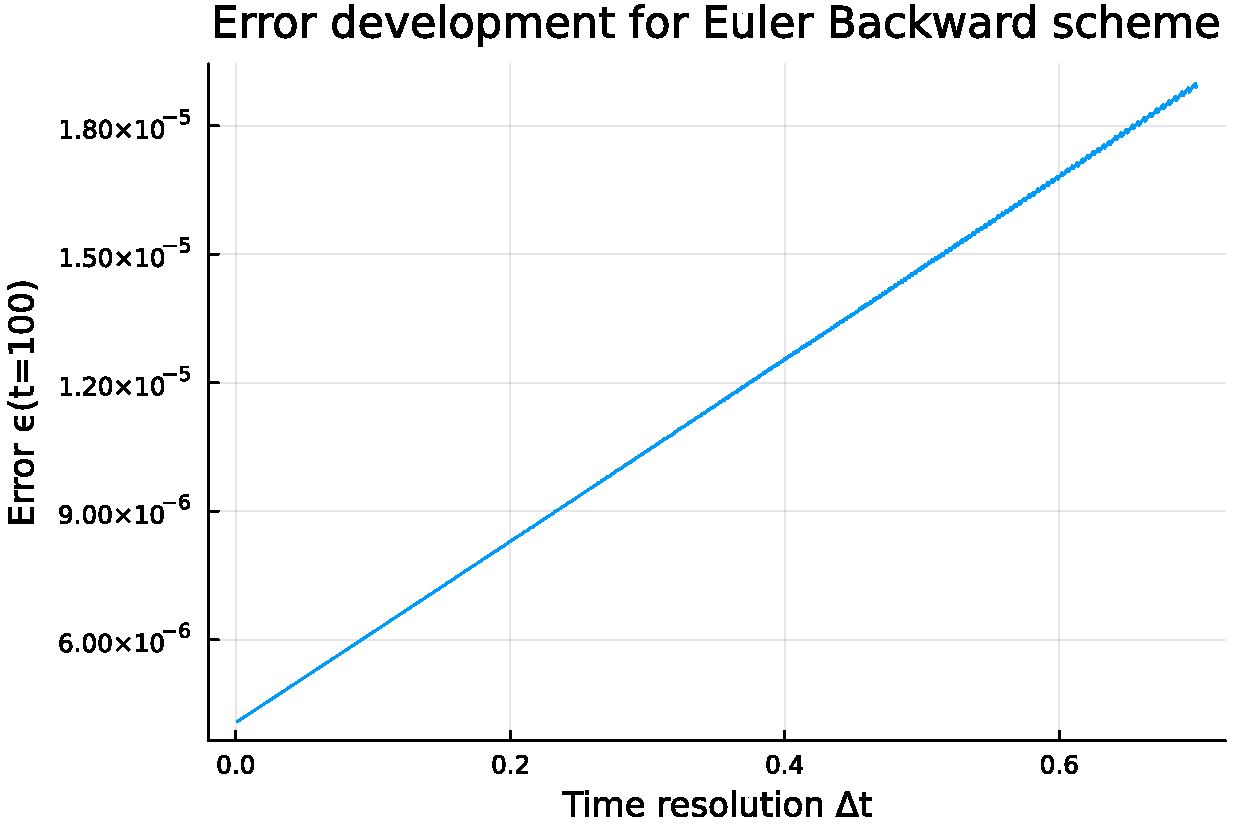
\includegraphics[width=\textwidth]{../saves_t2/error_development_eb.pdf}
	\end{subfigure}
	\hfill
	\begin{subfigure}[b]{0.49\textwidth}
		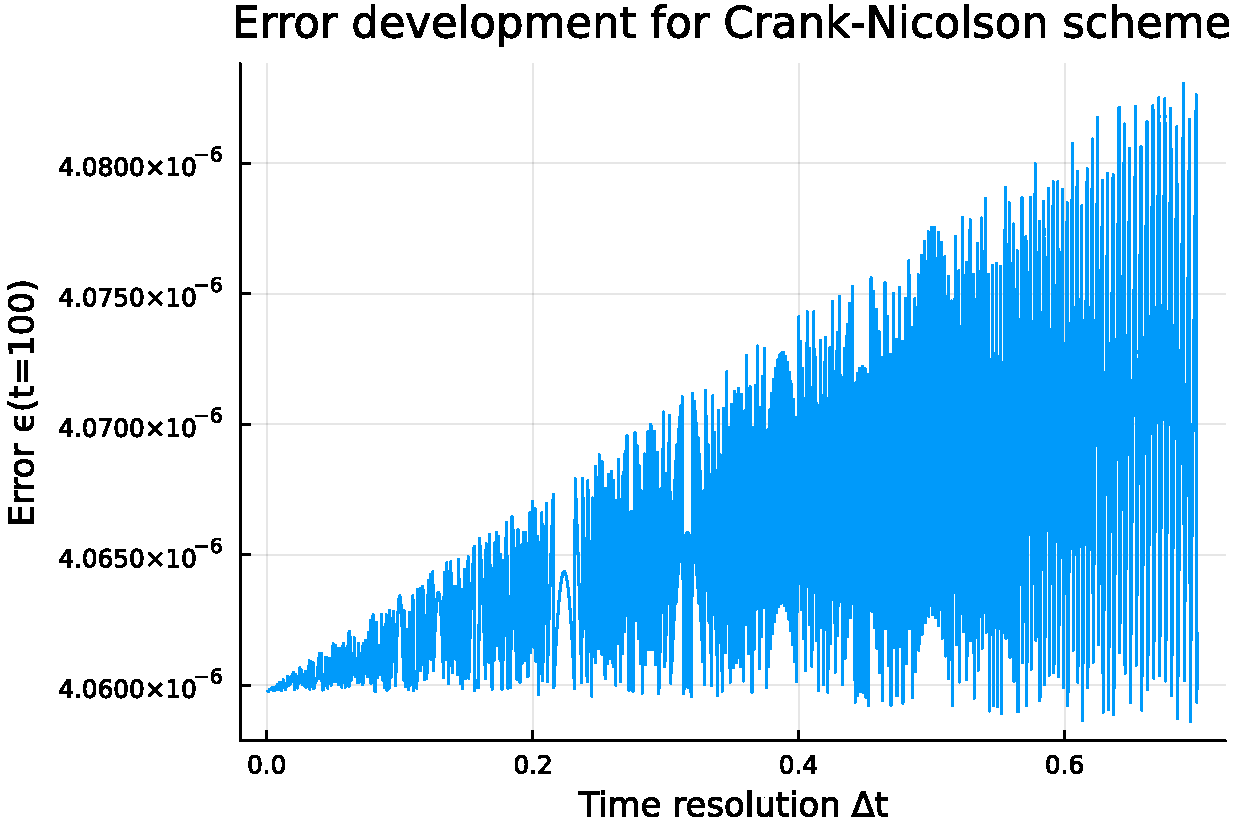
\includegraphics[width=\textwidth]{../saves_t2/error_development_cn.pdf}
	\end{subfigure}
	\hfill
	\begin{subfigure}[b]{0.49\textwidth}
		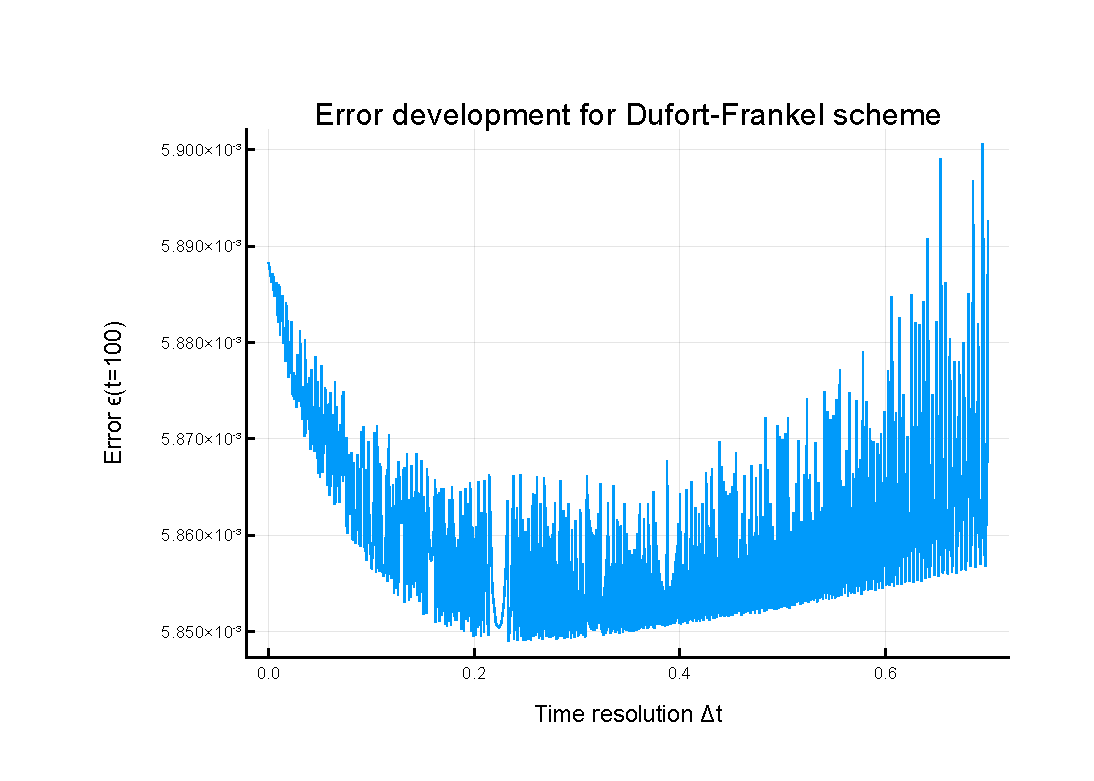
\includegraphics[width=\textwidth]{../saves_t2/error_development_df.pdf}
	\end{subfigure}
	\hfill
	\caption{}
	\label{fig:all_trunc_errors}
\end{figure}


\section{Solitons}





%----------------------------------------------------------------------------------------
%	DISCUSSION
%----------------------------------------------------------------------------------------

% \section{Discussion}



%----------------------------------------------------------------------------------------
%	BIBLIOGRAPHY
%----------------------------------------------------------------------------------------

% \printbibliography % Output the bibliography

%----------------------------------------------------------------------------------------

\end{document}